\documentclass[11pt,a4paper,fleqn,twoside]{article}
% Uncomment the following line to allow the usage of graphics (.png, .jpg)
\usepackage[pdftex]{graphicx}
\usepackage[a4paper,inner=2.2cm,outer=2.2cm,bottom=2.2cm,headheight=1cm]{geometry} % to change the page dimensions
% Comment the following line to NOT allow the usage of umlauts
\usepackage[utf8]{inputenc}
\usepackage[T1]{fontenc}
\usepackage{hyperref}

\usepackage{titling}
\renewcommand{\droptitle}{50pt}

\pretitle{%
  \begin{center}
  \LARGE
  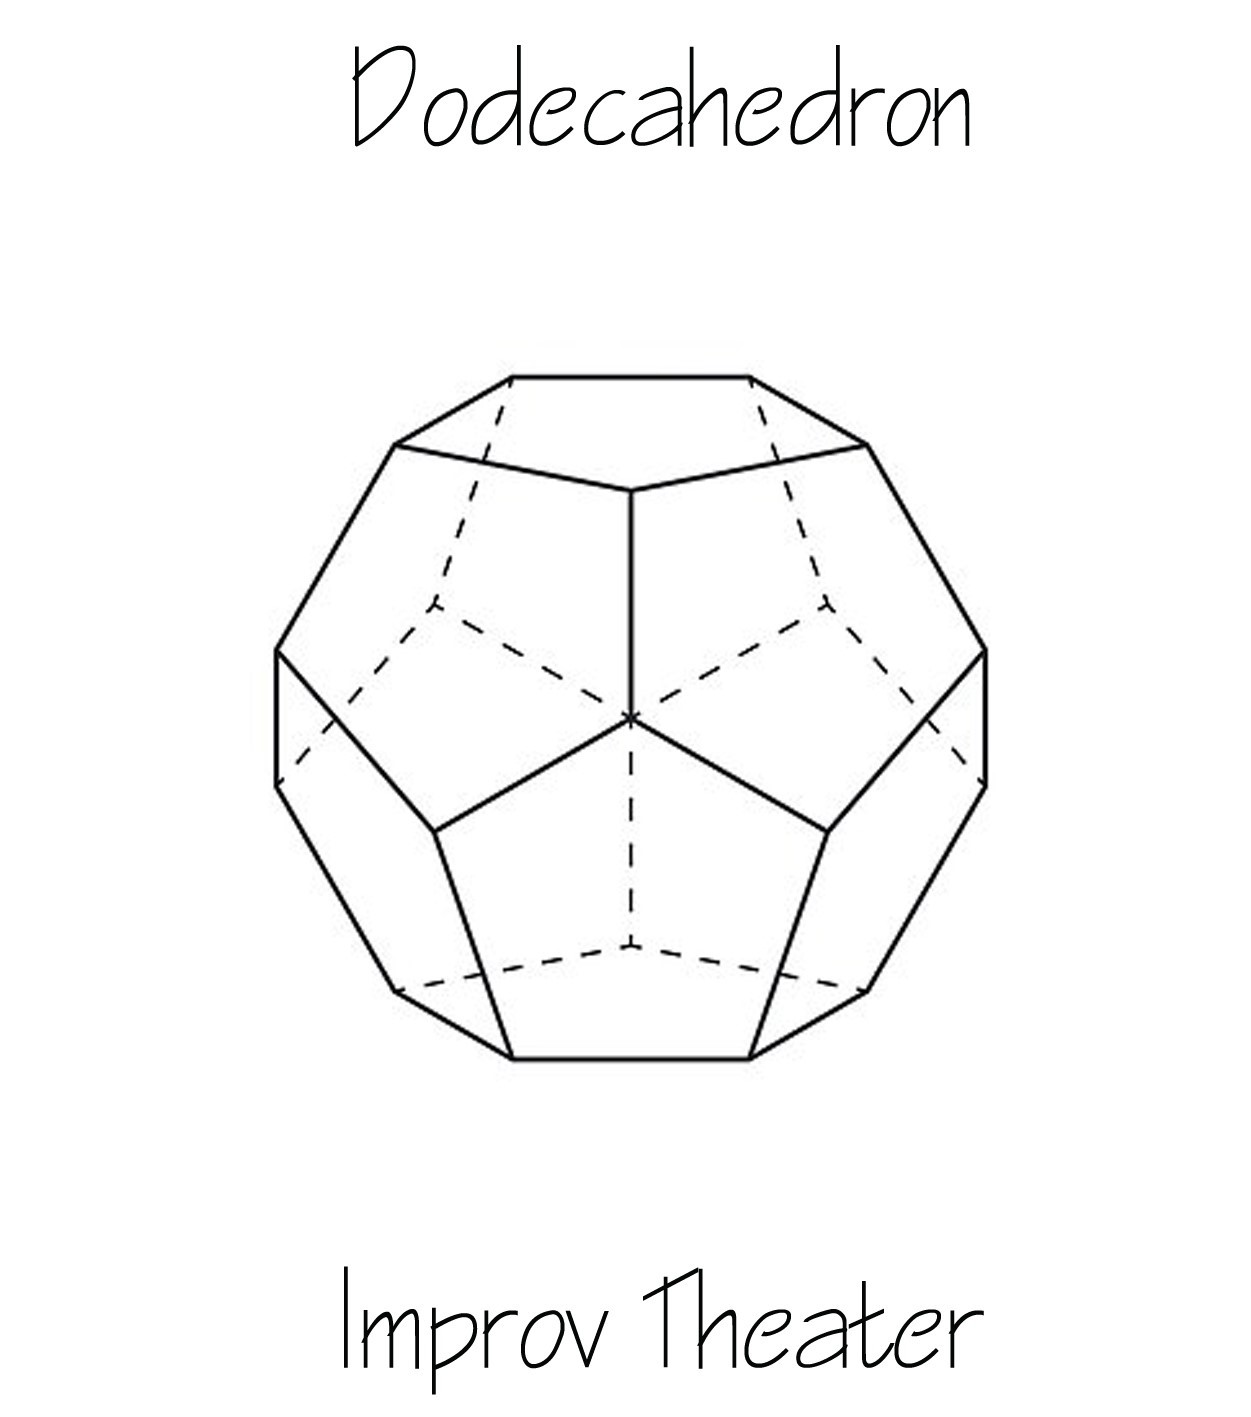
\includegraphics[width=0.6 \textwidth]{logo}\\[\bigskipamount]
}
\posttitle{\end{center}}
\title{Diary for a new theater group}
\author{Dodecahedron Improv Group}

\begin{document}
\maketitle
\clearpage
\tableofcontents
%%%%%%%%%%%%%%%%%%%%%%%%%%%%
% Sections
\clearpage

\section{Introduction}

We are the Dodecahedron Improv Theater (DIT) group, a non-profit group of students and young professionals from different paths of life who gather on a weekly basis to learn and rehearse theater improvisation. Our group was brought to life in July 2017. We meet on weekly basis for rehearsals at ETH Zürich zentrum, usually on Wednesdays. One can find more updated information about us in our \href{https://www.facebook.com/dodecahedronimprovtheater/}{Facebook page}.

\subsection{Improvisational theater, Improv}

The improvisational theater or, also called ``Improv'' is just another form of theater. It just have the particularity that there is not predefined script of the story that it is going to be performed on the stage. Instead, it will be the actors of improvisers the ones in charge of creating it, on the go. In Improv the people on the stage are the actors, producers and directors of the ongoing plot, everything at the same time.

Their stories will usually be motivated by some external interaction. In occasions the audience will provide some aspect of the story to be told that will guide the improvisers, for example a relationship between characters, the place will the action will take place or a general idea that shall be translated into a plot. 

\section{Sessions diary}

\subsection{Wednesday 27th March}

Bla blabla

\end{document}